% !TEX program = lualatex
\documentclass[aspectratio=169]{beamer}
\usepackage{beamerthemeihme}
\usepackage{bm}
\usepackage{tabularray}
\usepackage{makecell}
\usepackage{tabularray}
\usepackage{tikz}
\usetikzlibrary{positioning}

\newcommand{\btVFill}{\vskip0pt plus 1filll}

\title{Raking Methods and Applications to Health Metrics}
\subtitle{2025 SIAM Annual Meeting}
\author{Ariane Ducellier, Peng Zheng, Aleksandr Aravkin}

\begin{document}

\begin{frame}
\titlepage
\end{frame}

\begin{frame}
	\frametitle{What is raking?}
	\begin{columns}
	\begin{column}{.5\textwidth}
		\centering
		\includegraphics[width=7cm, trim={4.5cm 18cm 9cm 4.5cm},clip]{raking_2D_before.pdf}
	\end{column}

	\begin{column}{.5\textwidth}
		Two categorical variables $X_1$ and $X_2$ taking $I$ and $J$ possible values.

		\vspace{1em}

		When summing the rows and columns of the table $y$, the observations $y_{ij}$ do not add up to the values in the margins $s_1$ and $s_2$.

		\begin{equation*}
		\sum_{i = 1}^I y_{ij} \neq s_{1j} \quad j = 1 , \cdots , J
		\end{equation*}

		\begin{equation*}
		\sum_{j = 1}^J y_{ij} \neq s_{2i} \quad i = 1 , \cdots , I
		\end{equation*}
	\end{column}
	\end{columns}
\end{frame}

\begin{frame}
	\frametitle{What is raking?}
	\begin{columns}
	\begin{column}{.5\textwidth}
		\centering
		\includegraphics[width=7cm, trim={4.5cm 18cm 9cm 4.5cm},clip]{raking_2D_after.pdf}
	\end{column}

	\begin{column}{.5\textwidth}
		After raking, the raked values $\beta_{ij}$ in the updated table $\beta$ sum correctly to the values in the margins $s_1$ and $s_2$.

		\begin{equation*}
		\sum_{i = 1}^I \beta_{ij} = s_{1j} \quad j = 1 , \cdots , J
		\end{equation*}

		\begin{equation*}
		\sum_{j = 1}^J \beta_{ij} = s_{2i} \quad i = 1 , \cdots , I
		\end{equation*}

		\vspace{1em}

		Note: For the problem to have a solution, we need the margins to be consistent:

		\begin{equation*}
		\sum_{j = 1}^J s_{1j} = \sum_{i = 1}^I s_{2i}
		\end{equation*}
	\end{column}
	\end{columns}
\end{frame}

\begin{frame}
	\frametitle{Global health example}
	\begin{itemize}
		\setlength\itemsep{2em}
		\item The observation table may be the number of obesity cases for each population group $i$ and each county $j$. The margins are the number of obesity cases for the entire population for each county $j$ and the number of cases for each population group $i$ for the entire state.
		\item For some reason (e.g. errors in data collection, the table is the output of a model that does not include the constraints on the margins), the partial sums on the observations do not match the margins.
		\item We trust more the margins than the observations.
	\end{itemize}
\end{frame}

\begin{frame}
	\frametitle{Raking as an optimization problem}
	\begin{itemize}
		\item[] $y \in \mathbb{R}^p$ is the vectorized observation table.
		\item[] $s \in \mathbb{R}^k$ are the known margins, i.e. the known partial sums on the table.
		\item[] $A \in \mathbb{R}^{k \times p}$ summarizes how to compute the partial sums.
		\item[] $\beta \in \mathbb{R}^p$ are the unknown raked values.
		\item[] $w \in \mathbb{R}^p$ are raking weights chosen by the user.
		\item[] $f^w$ is a separable, derivable, positive, strictly convex function chosen by the user.
	\end{itemize}

	\begin{equation*}
	\min_{\beta \in \mathbb{R}^p} f^w \left( \beta ; y \right) \quad \text{s.t.} \quad A \beta = s \quad \text{with} \quad f^w \left( \beta ; y \right) = \sum_{i = 1}^p w_i f_i \left( \beta_i , y_i \right) \quad \text{and e.g.} \quad A = \begin{pmatrix} I_J \otimes \mathbb{1}_I^T \\ \mathbb{1}_J^T \otimes I_I \end{pmatrix}
	\end{equation*}

	\vspace{2em}

	Note: We need to ensure that all the constraints are consistent and we trim the redundant constraints such that $\text{rank} \left( A \in \mathbb{R}^{k \times p} \right) = k \leq p $.
\end{frame}

\begin{frame}
	\frametitle{Dual formulation}
	\begin{equation*}
	\mathcal{P}: \quad \min_{\beta \in \mathbb{R}^p} f^w \left( \beta , y \right) \quad \text{s.t} \quad A \beta = s
	\end{equation*}

	\begin{equation*}
	\mathcal{L}: \quad f^w \left( \beta , y \right) + \lambda^T \left( A \beta - s \right)
	\end{equation*}

	\begin{equation*}
	\mathcal{D}: \quad \min_{\lambda \in \mathbb{R}^k} f^{w*} \left( - A^T \lambda \right) + \lambda^T s
	\end{equation*}

	\vspace{2em}

	As $k \leq p$, we decrease the dimension of the problem by using the dual formulation instead of the primal formulation.

	\vspace{1em}

	We solve the dual problem using Newton's method.
\end{frame}

\begin{frame}
	\frametitle{Common distance functions}
	\begin{footnotesize}
	\begin{center}
	\begin{tabular}{| l | c c c |} 
	\hline
	& Distance $f_i \left( \beta_i ; y_i \right)$ & Solution & Note \\ 
	\hline
	$\chi^2$ & $\frac{1}{2 y_i} \left( \beta_i - y_i \right)^2$ & $\beta^* = y \odot \left( 1 - \frac{1}{w} \odot A^T \lambda^* \right)$ & \makecell[l]{Solved in 1 iteration.} \\ 
	\hline
	Entropic & $\beta_i \log \left( \frac{\beta_i}{y_i} \right) - \beta_i + y_i$ & $\beta^* = y \odot \exp \left( - \frac{1}{w} \odot A^T \lambda^* \right)$ & \makecell[l]{The raked values have \\ the same sign as \\ the initial observations.} \\
	\hline
	Logit & $\left( \beta_i - l_i \right) \log \frac{ \beta_i - l_i}{y_i - l_i} + \left( h_i - \beta_i \right) \log \frac{ h_i - \beta_i}{h_i - y_i}$ & $\beta^* = \frac{l \odot \left( h - y \right) + h \odot \left( y - l \right) \odot e^{ - \frac{1}{w} \odot A^T \lambda^*}}{ \left( h - y \right) + \left( y - l \right) \odot e^{ - \frac{1}{w} \odot A^T \lambda^*}}$ & \makecell[l]{The raked values stay \\ between $l_i$ and $h_i$ \\ when we rake \\ prevalence observations.} \\
	\hline
	\end{tabular}
	\end{center}
	\end{footnotesize}
\end{frame}

\begin{frame}
	\frametitle{Prior ordinal constraints}
	\begin{columns}
	\begin{column}{.4\textwidth}
	We are given observations and margins for $n$ different years $\rightarrow$ We can solve $n$ independent raking problems:

	\vspace{2em}

	\begin{equation*}
	\begin{aligned}
	& \min_{\beta_1 \in \mathbb{R}^p} f^w \left( \beta_1 , y_1 \right) \quad \text{s.t} \quad A_1 \beta_1 = s_1 \\
	& \vdots \\
	& \min_{\beta_n \in \mathbb{R}^p} f^w \left( \beta_n , y_n \right) \quad \text{s.t} \quad A_n \beta_n = s_n
	\end{aligned}
	\end{equation*}
	\end{column}

	\begin{column}{.6\textwidth}
		\centering
		\includegraphics[width=8cm, trim={4.5cm 13cm 5cm 4.5cm},clip]{raking_2D_multiple.pdf}
	\end{column}
	\end{columns}
\end{frame}

\begin{frame}{Prior ordinal constraints}
	\begin{columns}

	\begin{column}{.5\textwidth}
		We want the raking process to preserve the sign of the trend observed between year $1$ and year $2$, year $2$ and year $3$, and so on and so forth until year $n$.

		\vspace{1em}

		$\left( n - 1 \right) p $ additional constraints must then be added:

		\vspace{1em}

		\begin{equation*}
		\begin{aligned}
		&\left( \beta_{1,i} - \beta_{2,i} \right) \left( y_{1,i} - y_{2,i} \right) \geq 0 \quad \forall i = 1 , \cdots , p \\
		& \vdots \\
		&\left( \beta_{n-1,i} - \beta_{n,i} \right) \left( y_{n-1,i} - y_{n,i} \right) \geq 0 \quad \forall i = 1 , \cdots , p
		\end{aligned}
		\end{equation*}
	\end{column}

	\begin{column}{.5\textwidth}
		The raking problem becomes:

		\begin{equation*}
		\begin{aligned}
		& \min_{\beta_1 , \cdots , \beta_n} f^w \left( \beta_1 , y_1 \right) + \cdots + f^w \left( \beta_n , y_n \right) \\
		& \text{s.t.} \quad \left\{
			\begin{aligned}
			& A_1 \beta_1 = s_1, \\
			& \cdots \\
			& A_n \beta_n = s_n, \\
			& - \left( \beta_1 - \beta_2 \right) \odot \left( y_1 - y_2 \right) \leq 0 \\
			& \cdots \\
			& - \left( \beta_{n-1} - \beta_n \right) \odot \left( y_{n-1} - y_n \right) \leq 0
			\end{aligned}
			\right.
		\end{aligned}
		\end{equation*}
	\end{column}
	\end{columns}
\end{frame}

\begin{frame}{Prior ordinal constraints}
	We end up with a minimization problem with the same form as before:

	\vspace{3em}

	\begin{columns}[t]

	\begin{column}{.45\textwidth}
		Inequality constraints
		\begin{equation*}
		\min_{\beta \in \mathbb{R}^{n p}} f^w \left( \beta , y \right) \quad \mbox{s.t.} \quad \left\{
		\begin{aligned}
		& A \beta = s, \\
		& C \beta \leq c
		\end{aligned}
		\right.
		\end{equation*}
		The feasible set may be empty. 
	\end{column}
	
	\begin{column}{.45\textwidth}
		Penalty
		\begin{equation*}
		\min_{\beta \in \mathbb{R}^{n p}} f^w \left( \beta , y \right) + L \left( c - C \beta , \alpha \right) \quad \mbox{s.t.} \quad A \beta = s
		\end{equation*}
		$\alpha$ is a penalty parameter and $L$ can be the logistic loss:
		\begin{equation*}
		L^{\text{logit}} \left( x \right) = \sum_{i = 1}^m \log \left( 1 + \exp \left( - x_i \right) \right)
		\end{equation*}
	\end{column}

	\end{columns}
\end{frame}

\begin{frame}
	\frametitle{Variance propagation}
	Given:

	\begin{itemize}
	\item $\Sigma_y \in \mathbb{R}^{p \times p}$, the covariance matrix of the observations vector $y$,
	\item $\Sigma_s \in \mathbb{R}^{k \times k}$, the covariance matrix of the margins vector $s$ and
	\item $\Sigma_{y s} \in \mathbb{R}^{p \times k}$, the covariance matrix of $y$ and $s$,
	\end{itemize}

	\vspace{1em}

	find:

	\begin{itemize}
	\item $\Sigma_{\beta^*} \in \mathbb{R}^{p \times p}$, the covariance matrix of the estimated raked values $\beta^*$.
	\end{itemize}
\end{frame}

\begin{frame}
	\frametitle{Variance propagation}
	The primal problem:

	\begin{equation*}
	\min_{\beta \in \mathbb{R}^p} \max_{\lambda \in \mathbb{R}^k} f^w \left( \beta , y \right) + L \left( c - C \beta , \alpha \right) + \lambda^T \left( A \beta - s \right) 
	\end{equation*}

	can also be written:

	\begin{equation*}
	F \left( \beta , \lambda ; y , s \right) = \begin{bmatrix} \nabla_\beta f^w \left( \beta , y \right) - C^T \nabla_x L \left( c - C \beta , \alpha \right) + A^T \lambda \\ A \beta - s \end{bmatrix} = 0
	\end{equation*}

	and has solution:

	\begin{equation*}
	\beta^* = \phi \left( y , s \right) \text{ with } \phi : \mathbb{R}^{p+k} \rightarrow \mathbb{R}^p
	\end{equation*}
\end{frame}

\begin{frame}
	\frametitle{Variance propagation}
	We get:

	\begin{equation*}
	\Sigma_{\beta^*} =  \phi'_{ys} \left( y , s \right) \Sigma \phi^{'T}_{ys} \left( y , s \right)
	\end{equation*}

	with:

	\begin{equation*}
	\phi'_{ys} \left( y , s \right) = \begin{pmatrix} \frac{\partial \beta^*}{\partial y} & \frac{\partial \beta^*}{\partial s} \end{pmatrix} = \begin{pmatrix} \frac{\partial \phi_1}{\partial y_1} \left( y , s \right) & \hdots & \frac{\partial \phi_1}{\partial y_p} \left( y , s \right) & \frac{\partial \phi_1}{\partial s_1} \left( y , s \right) & \hdots & \frac{\partial \phi_1}{\partial s_k} \left( y ; s \right) \\ \vdots & & \vdots & \vdots & & \vdots \\ \frac{\partial \phi_p}{\partial y_1} \left( y , s \right) & \hdots & \frac{\partial \phi_p}{\partial y_p} \left( y , s \right) & \frac{\partial \phi_p}{\partial s_1} \left( y , s \right) & \hdots & \frac{\partial \phi_p}{\partial s_k} \left( y , s \right) \end{pmatrix}
	\end{equation*}

	and:

	\begin{equation*}
	\Sigma = \begin{pmatrix} \Sigma_y & \Sigma_{ys} \\ \Sigma_{ys}^T & \Sigma_s \end{pmatrix}
	\end{equation*}
\end{frame}

\begin{frame}
	\frametitle{Variance propagation}
	Implicit Function Theorem: When differentiating the primal problem $F \left( y , s ; \phi \left( y , s \right) \right) = 0$ at the solution $\left( \beta^* , \lambda^* \right)$, we get:

	\begin{equation*}
	\left[ D_{\beta , \lambda} F \left( y , s ; \beta^* , \lambda^* \right) \right] \left[ D_{y , s} \phi \left( y , s \right) \right] + \left[ D_{y , s} F \left( y , s ; \beta^* , \lambda^* \right) \right] = 0
	\end{equation*}

	\vspace{1em}

	Knowing $D_{\beta , \lambda} F$ and $D_{y , s} \phi$, we can compute:

	\begin{equation*}
	D_{y , s} \phi = \begin{pmatrix} \frac{\partial \beta^*}{\partial y} & \frac{\partial \beta^*}{\partial s} \\ \frac{\partial \lambda^*}{\partial y} & \frac{\partial \lambda^*}{\partial s} \end{pmatrix} \text{ and } \phi'_{ys} \left( y , s \right) = \begin{pmatrix} \frac{\partial \beta^*}{\partial y} & \frac{\partial \beta^*}{\partial s} \end{pmatrix}
	\end{equation*}

	We have:

	\begin{equation*}
	D_{\beta , \lambda} F = \begin{pmatrix} \nabla^2_\beta f^w \left( \beta^* , y \right) + C^T \nabla_{x^2} L \left( c - C \beta^* , \alpha \right) C & A^T \\ A & 0_{k \times k} \end{pmatrix}
	\end{equation*}

\end{frame}

\begin{frame}
	\frametitle{Variance propagation}
	We denote:

	\begin{equation*}
	\left[ A * b \right]_{ij} = \sum_{j = 1}^n A_{ijk} b_j \quad \text{for} \quad A \in \mathbb{R}^{m \times n \times p} \quad \text{,} \quad \beta \in \mathbb{R}^n \quad \text{and} \quad A * b \in \mathbb{R}^{m \times p}
	\end{equation*}

	\begin{equation*}
	\left[ \nabla_y A \right]_{ijk} = \frac{\partial A_{ij} \left( y \right)}{\partial y_k}
	\end{equation*}

	We get:

	\begin{equation*}
	D_{y , s} F = \begin{pmatrix} \nabla^2_{\beta y} f^w \left( \beta^* ; y \right) - \left[ \nabla_y C^T \right] \nabla_x L \left( c - C \beta^* , \alpha \right) + C^T \nabla_x^2 L \left( c - C \beta^* , \alpha \right) \left[ \nabla_y C * \beta \right] & 0_{p \times k} \\ 0_{k \times p} & - I_{k \times k} \end{pmatrix}
	\end{equation*}
\end{frame}

\begin{frame}
	\frametitle{Results}
	\centering
	Females, age 35-40, population group AIAN, county 534 (Hawaii)

	\vspace{1em}

	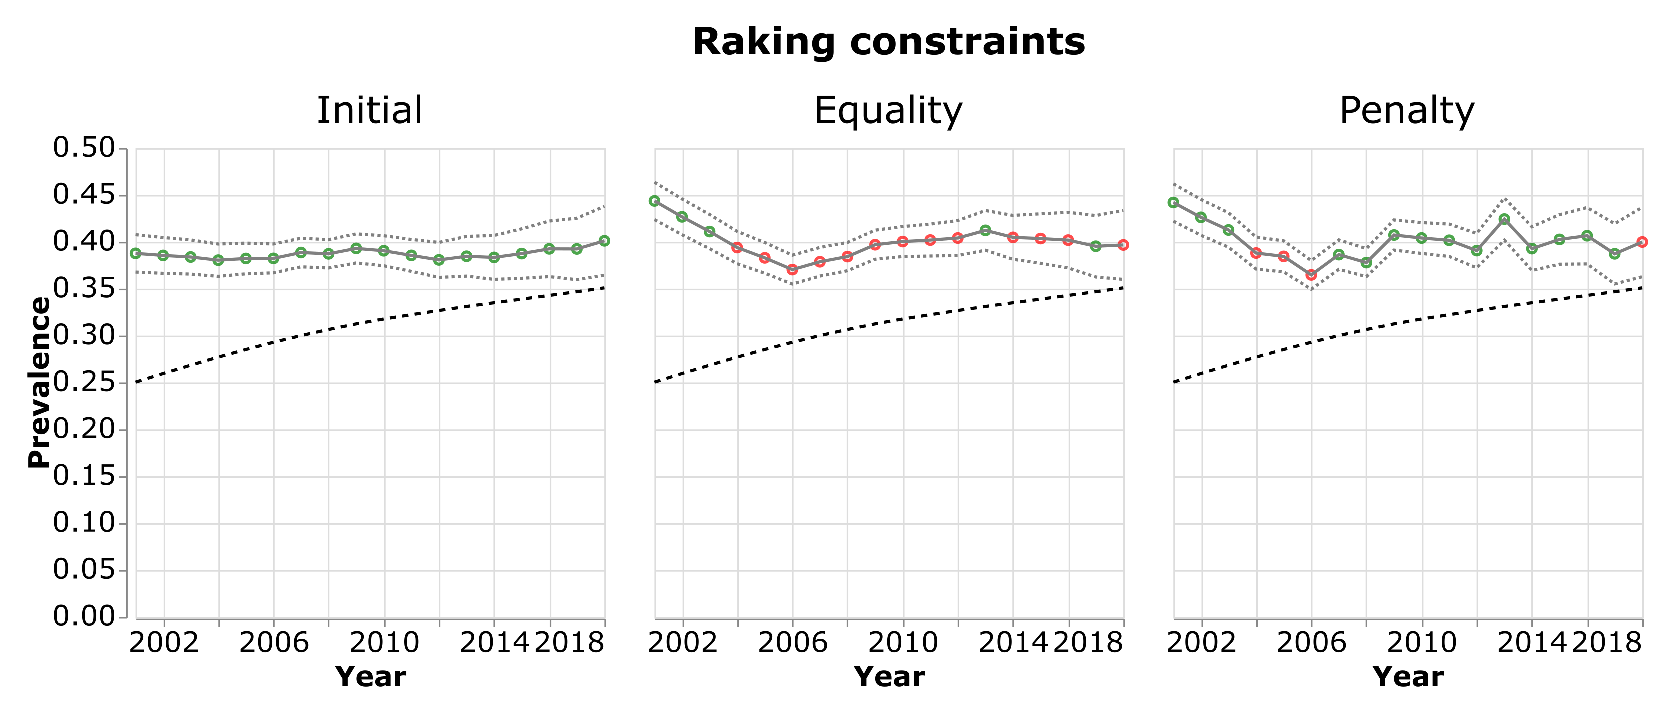
\includegraphics[width=12cm]{obesity_2_35_6_534.eps}
\end{frame}

\begin{frame}
	\frametitle{Results}
	\centering
	Females, age 35-40, population group API, county 532 (Hawaii), year 2011

	\vspace{1em}

	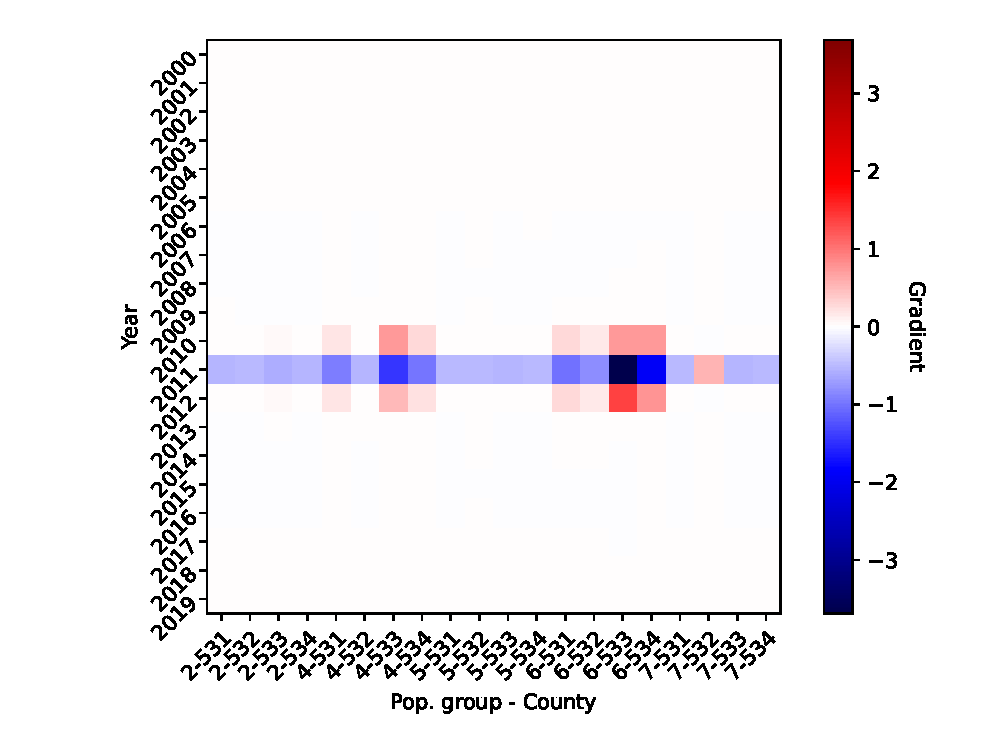
\includegraphics[width=8cm]{gradient_2_35_7_532_2011.eps}
\end{frame}

\begin{frame}
\btVFill
\center{\Huge{Questions?}}
\btVFill
PyPI: \href{https://pypi.org/project/raking/}{https://pypi.org/project/raking/}

GitHub: \href{https://github.com/ihmeuw-msca/raking}{https://github.com/ihmeuw-msca/raking}
\end{frame}

\end{document}